\documentclass[11pt, a4paper]{article}
%\usepackage{proj1}
\usepackage{natbib}
\usepackage{fancyhdr}  
\usepackage{subcaption}
\usepackage{caption}
\usepackage{graphicx}
\usepackage{numprint}
\usepackage{multirow}
\linespread{1.25} 
\setlength{\parindent}{0cm}
\graphicspath{{Images/}}
\usepackage{hyperref}
\usepackage{amsmath}
\usepackage{amsfonts}
\usepackage{amssymb}
\usepackage{amsthm}
\usepackage{mathtools}
\usepackage{commath}
\usepackage{bbm}

%\usepackage[sc,osf]{mathpazo}
\usepackage{subcaption}
\usepackage[a4paper, top=1in, left=1.0in, right=1.0in, bottom=1in, includehead, includefoot]{geometry} %Usually have top as 1in

\usepackage{listings}
\usepackage{color} %red, green, blue, yellow, cyan, magenta, black, white
\definecolor{mygreen}{RGB}{28,172,0} % color values Red, Green, Blue
\definecolor{mylilas}{RGB}{170,55,241}


\hypersetup{colorlinks,linkcolor={black},citecolor={blue},urlcolor={black}}
\usepackage{color}
\urlstyle{same}


\theoremstyle{definition}
\newtheorem{definition}{Definition}[section]

%\newcommand{\Sta}{\rho}
\newcommand{\adja}{q_a}
\newcommand{\adjb}{q_b}
\newcommand{\adjaB}{q_{a,\partial \Omega}}
\newcommand{\adjbB}{q_{b,\partial \Omega}}
%\newcommand{\Con}{u}
\newcommand{\ra}{\rho_a}
\newcommand{\rb}{\rho_b}
\newcommand{\w}{\mathbf{w}}
\newcommand{\Stav}{\mathbf{v}}
\newcommand{\Adja}{\mathbf{p}}
\newcommand{\Adjb}{q}
\newcommand{\Adjc}{{p}_{\partial \Sigma}}
\newcommand{\Con}{\mathbf{f}}
\newcommand{\n}{\mathbf{n}}
\newcommand{\h}{\mathbf{h}}
\newcommand{\K}{\mathbf{K}}


\pagenumbering{gobble}
\begin{document}
	\section{Multiple Species}
	We choose two species, impose a flow in opposite directions, repulsion between the species and attraction within the species. 
	Number of points are $n = 30$, $N = 50$. We run time from zero to $0.5$.
	If only flow is imposed, nothing can be observed, since the channel is periodic. Therefore, we choose $ \kappa = -1$ and $ \tilde \kappa = 1$. 
	The result can be seen in Figures \ref{F1a} and \ref{F1b}. The initial condition for species one is uniform, while the initial condition for species two is a cosine wave. This shows that the initial condition matters for the resulting structure, as expected. 
	\begin{figure}[h]
		\centering
		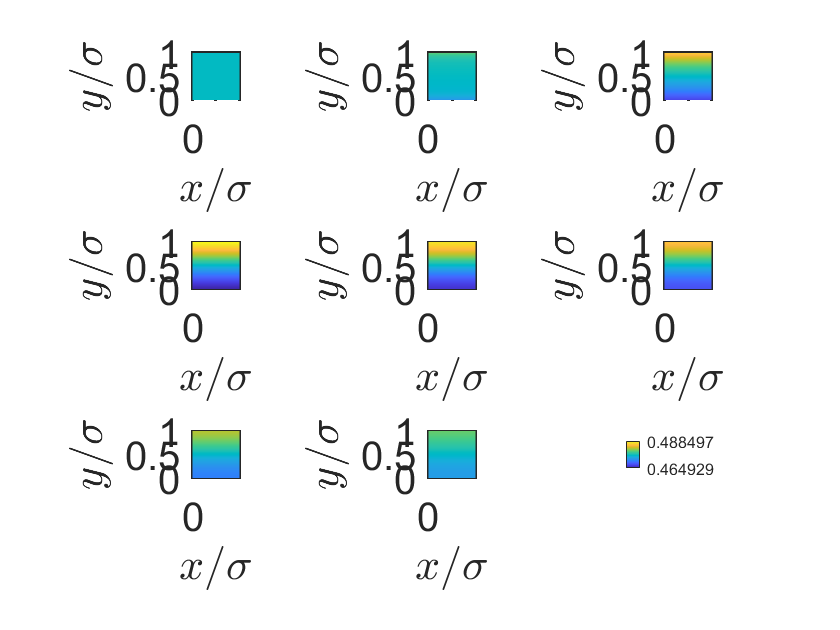
\includegraphics[scale=0.6]{Spec1.png}
		\caption{Species one over a time interval $[0,0.5]$} 
		\label{F1a}
	\end{figure}
		\begin{figure}[h]
		\centering
		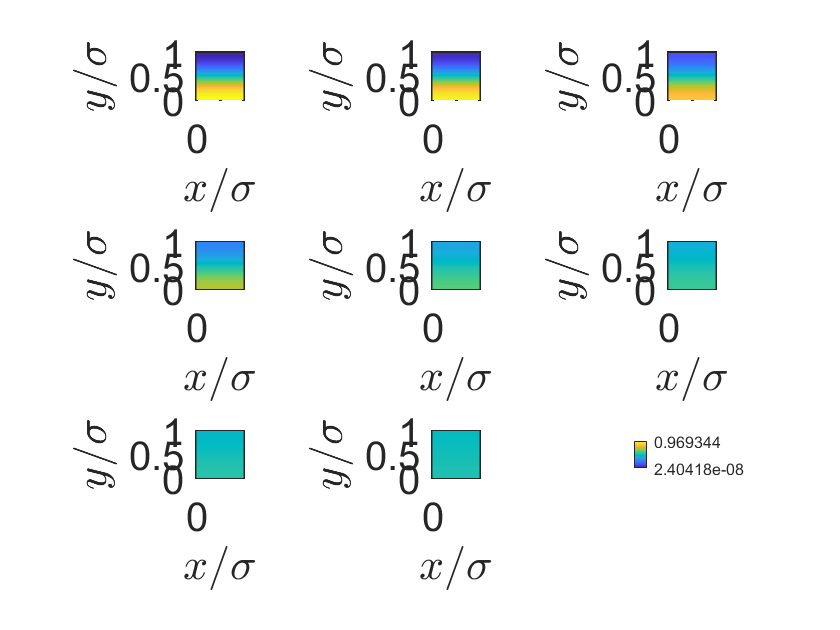
\includegraphics[scale=0.6]{Spec2.png}
		\caption{Species two over a time interval $[0,0.5]$} 
		\label{F1b}
	\end{figure}
	After running a few examples, we see that over time the diffusion takes over and is stronger than the interaction. Therefore, I choose to sun the problem with $D_0 = 0.1$, $\kappa = -1$, $\tilde \kappa = 2$ and the initial conditions to be sine and cosine waves with more oscillations. I plot times one to eight in $30$, see Figures \ref{F2a} and \ref{F2b}. The odd thing is that both of the species have a cluster on the bottom.
	\begin{figure}[h]
	\centering
	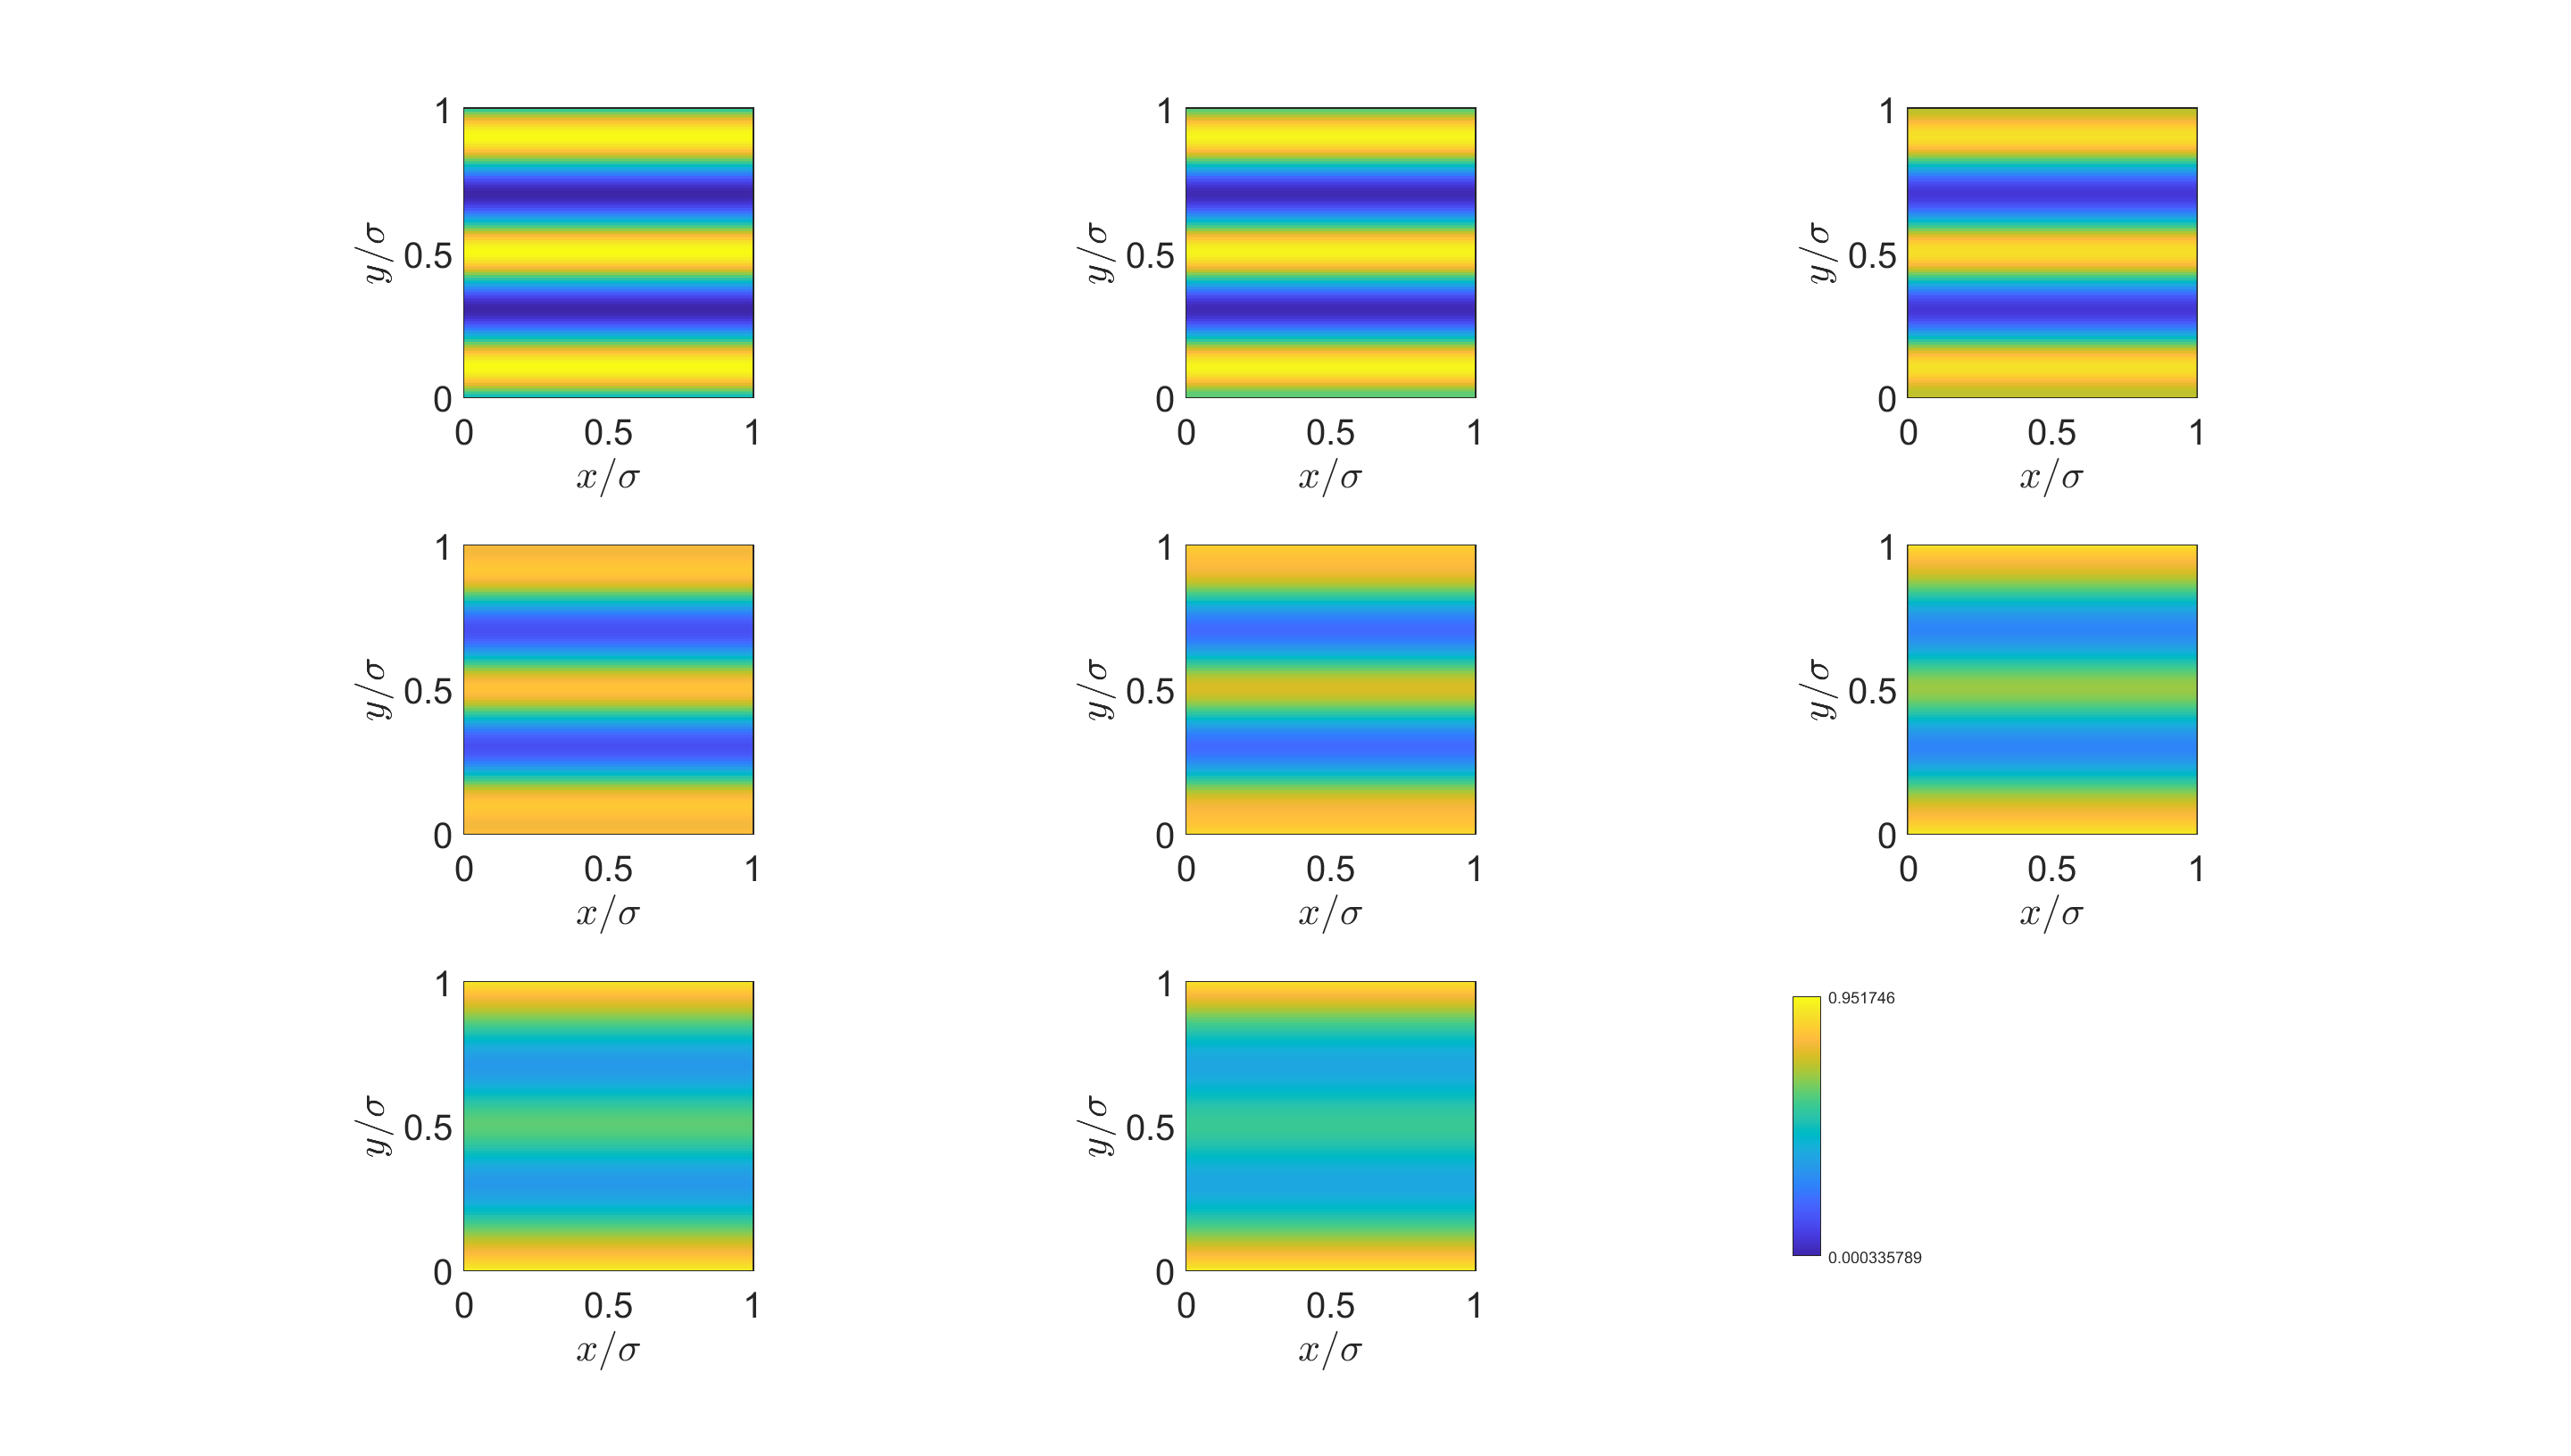
\includegraphics[scale=0.25]{Weird1.png}
	\caption{Ex1: Species one at times 1 to 8 out of 30, $\rho_0$ sine wave} 
	\label{F2a}
	\end{figure}
	\begin{figure}[h]
		\centering
		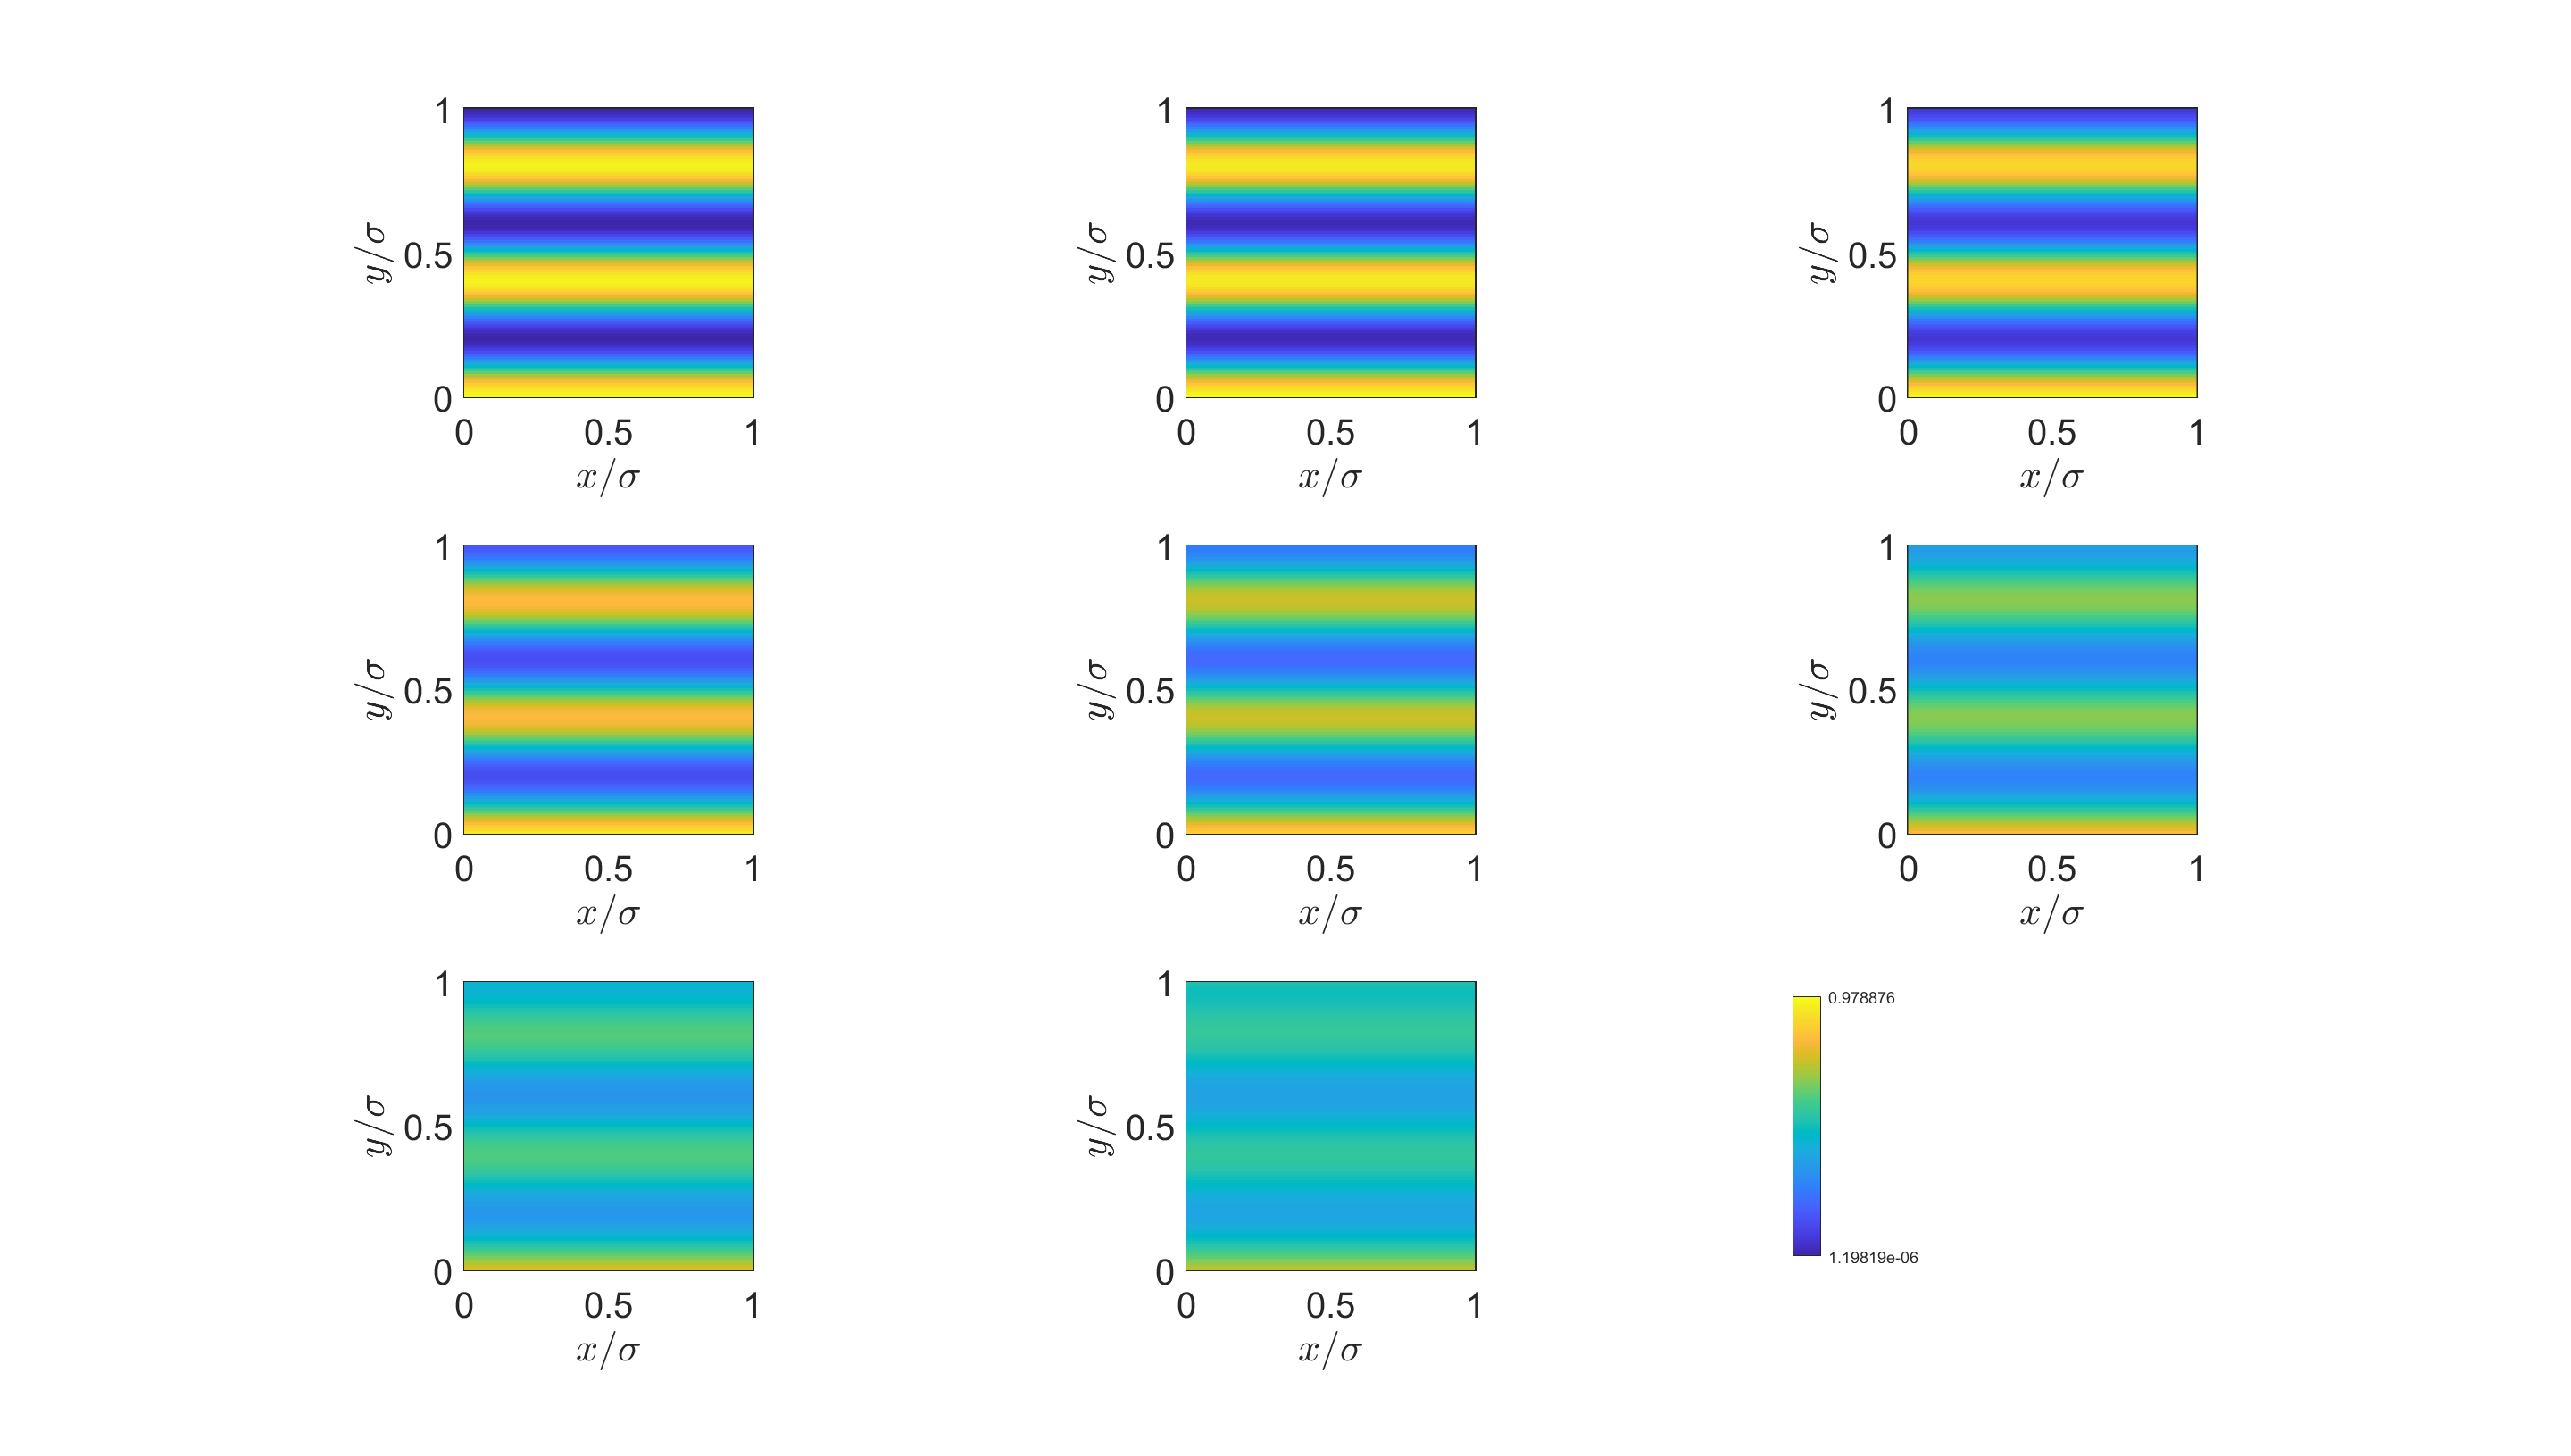
\includegraphics[scale=0.25]{Weird2.png}
		\caption{Ex1: Species two at times 1 to 8 out of 30, $\rho_0$ cosine wave} 
		\label{F2b}
	\end{figure}
	If we do the same thing but with one species having a constant initial condition, while the other species has a cosine wave as initial condition, this can be observed even more, see Figures \ref{F2c} and \ref{F2d}.
	\begin{figure}[h]
		\centering
		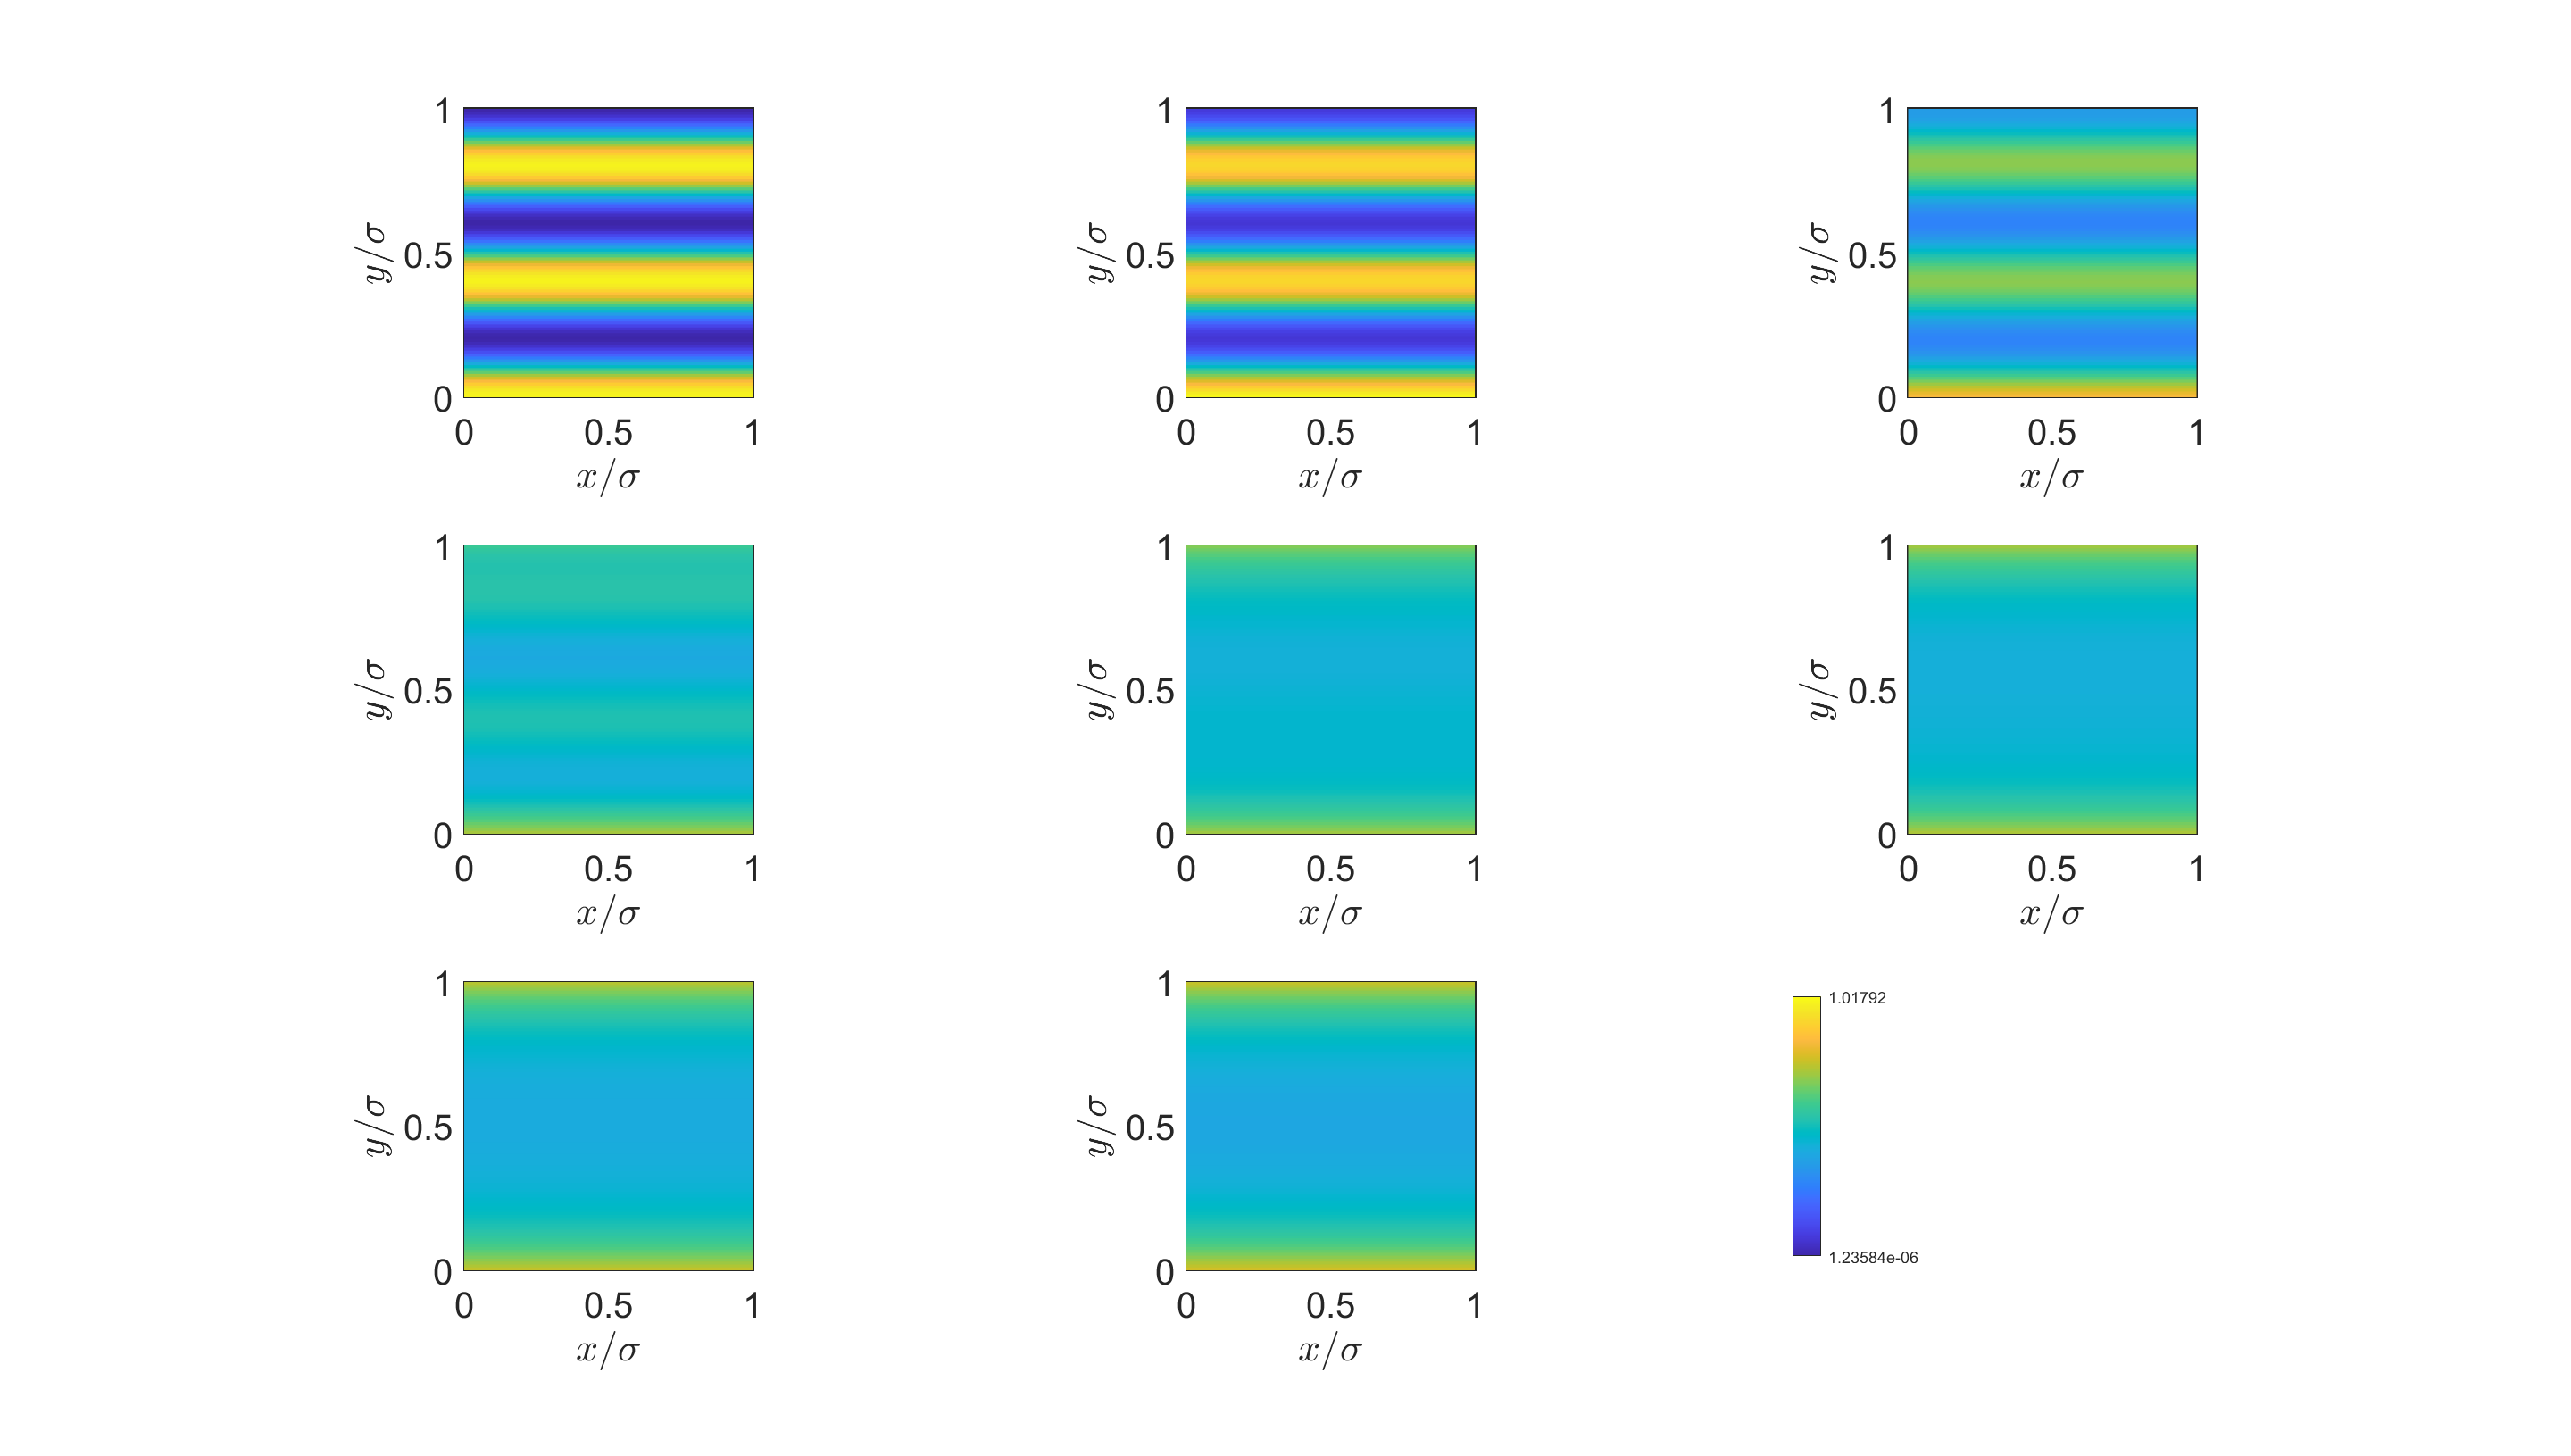
\includegraphics[scale=0.25]{Weird3.png}
		\caption{Ex2: Species one, full time horizon, $\rho_0$ constant ones} 
		\label{F2c}
	\end{figure}
	\begin{figure}[h]
		\centering
		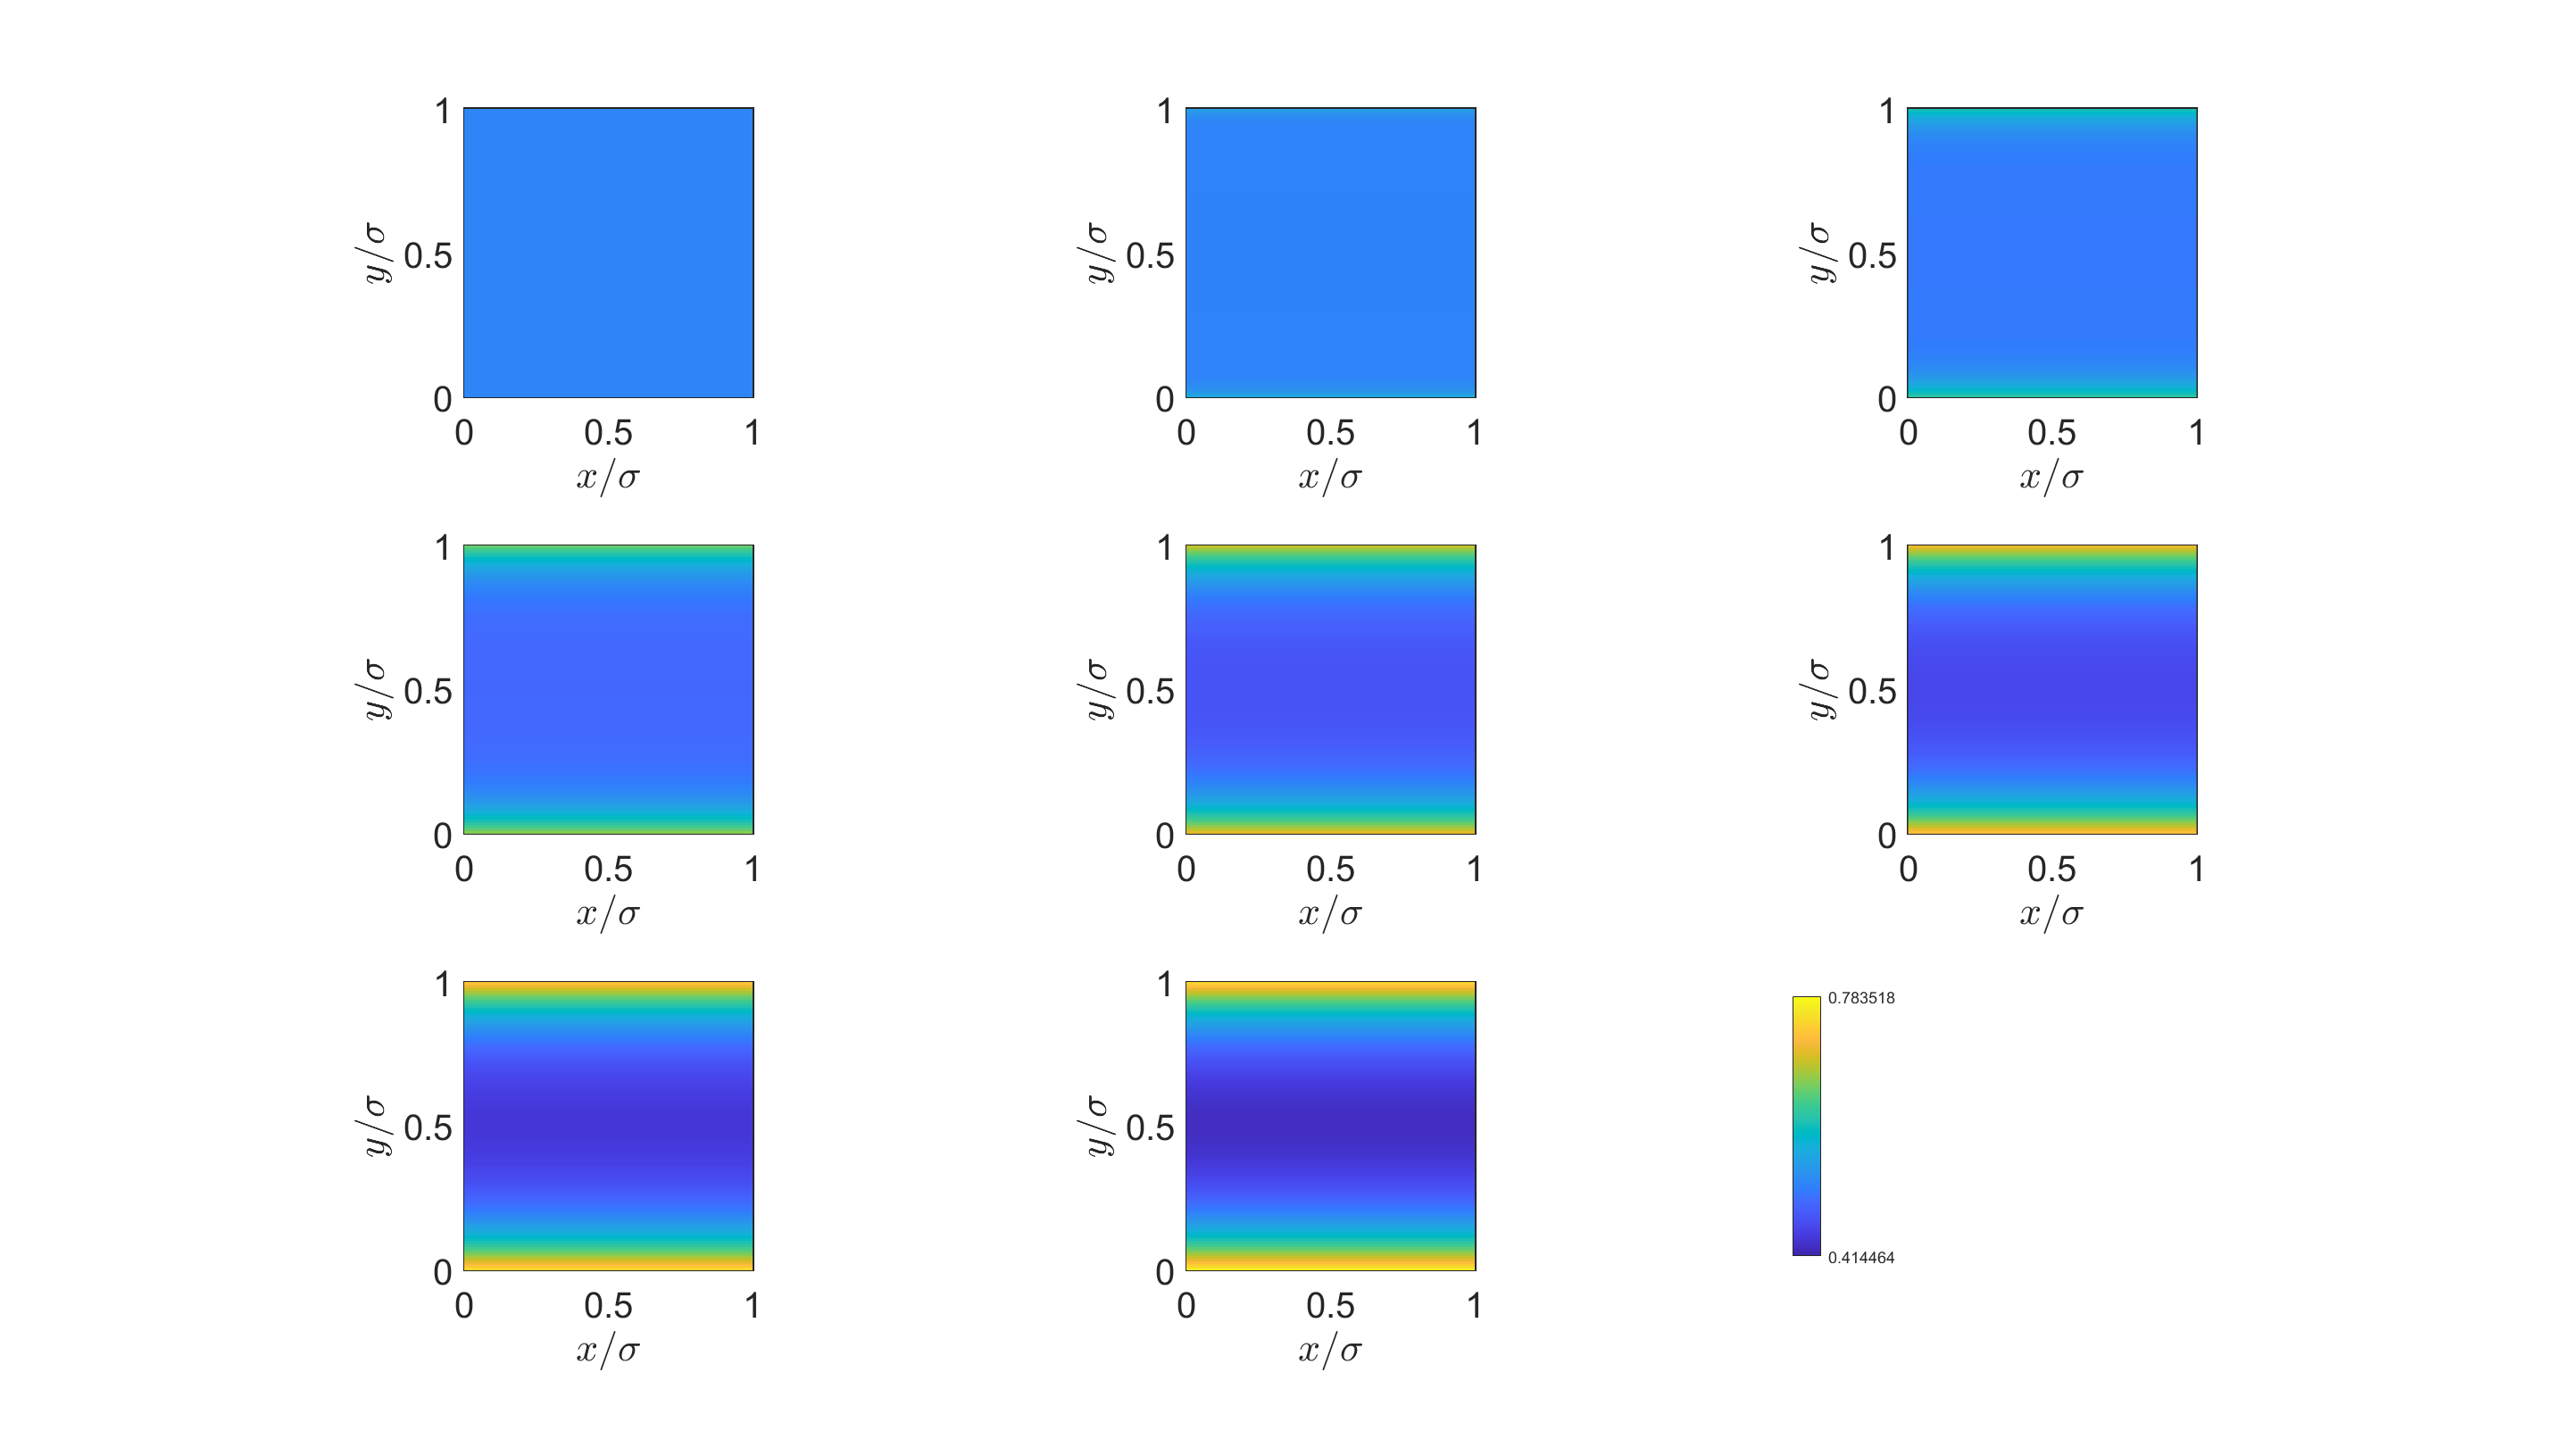
\includegraphics[scale=0.25]{Weird4.png}
		\caption{Ex2: Species two, full time horizon, $rho_0$ cosine wave} 
		\label{F2d}
	\end{figure}

\section{Sedimentation Optimization}
We choose the target with the external potential strength $ a = 0.1$ and the forward problem with $a = 0.05$. We expect that the flow control will have to push downward to complement the external potential, which is weaker than the one that created the target distribution. The results are displayed in Figures \ref{F3a} and \ref{F3b}.$J_{FW} = 0.1716$ and $J_{Opt} = 1.9866$.
In particular, in both cases $J_1 = 0.3432$, but in the forward problem $J_2 = 0$ and in the optimization problem $J_2 = 3.6300 \times 10^3$. This is with $\beta = 10^{-3}$ so the changes in magnitude are quite large. Maybe that introduces some error?\\
We run the same setup with $\beta = 10^{-1}$ and get $J_{FW} = 0.2417$ and $J_{Opt} = 0.2636$. This is still wrong but not as significantly. There might still be a mistake in the derivation.
	\begin{figure}[h]
	\centering
	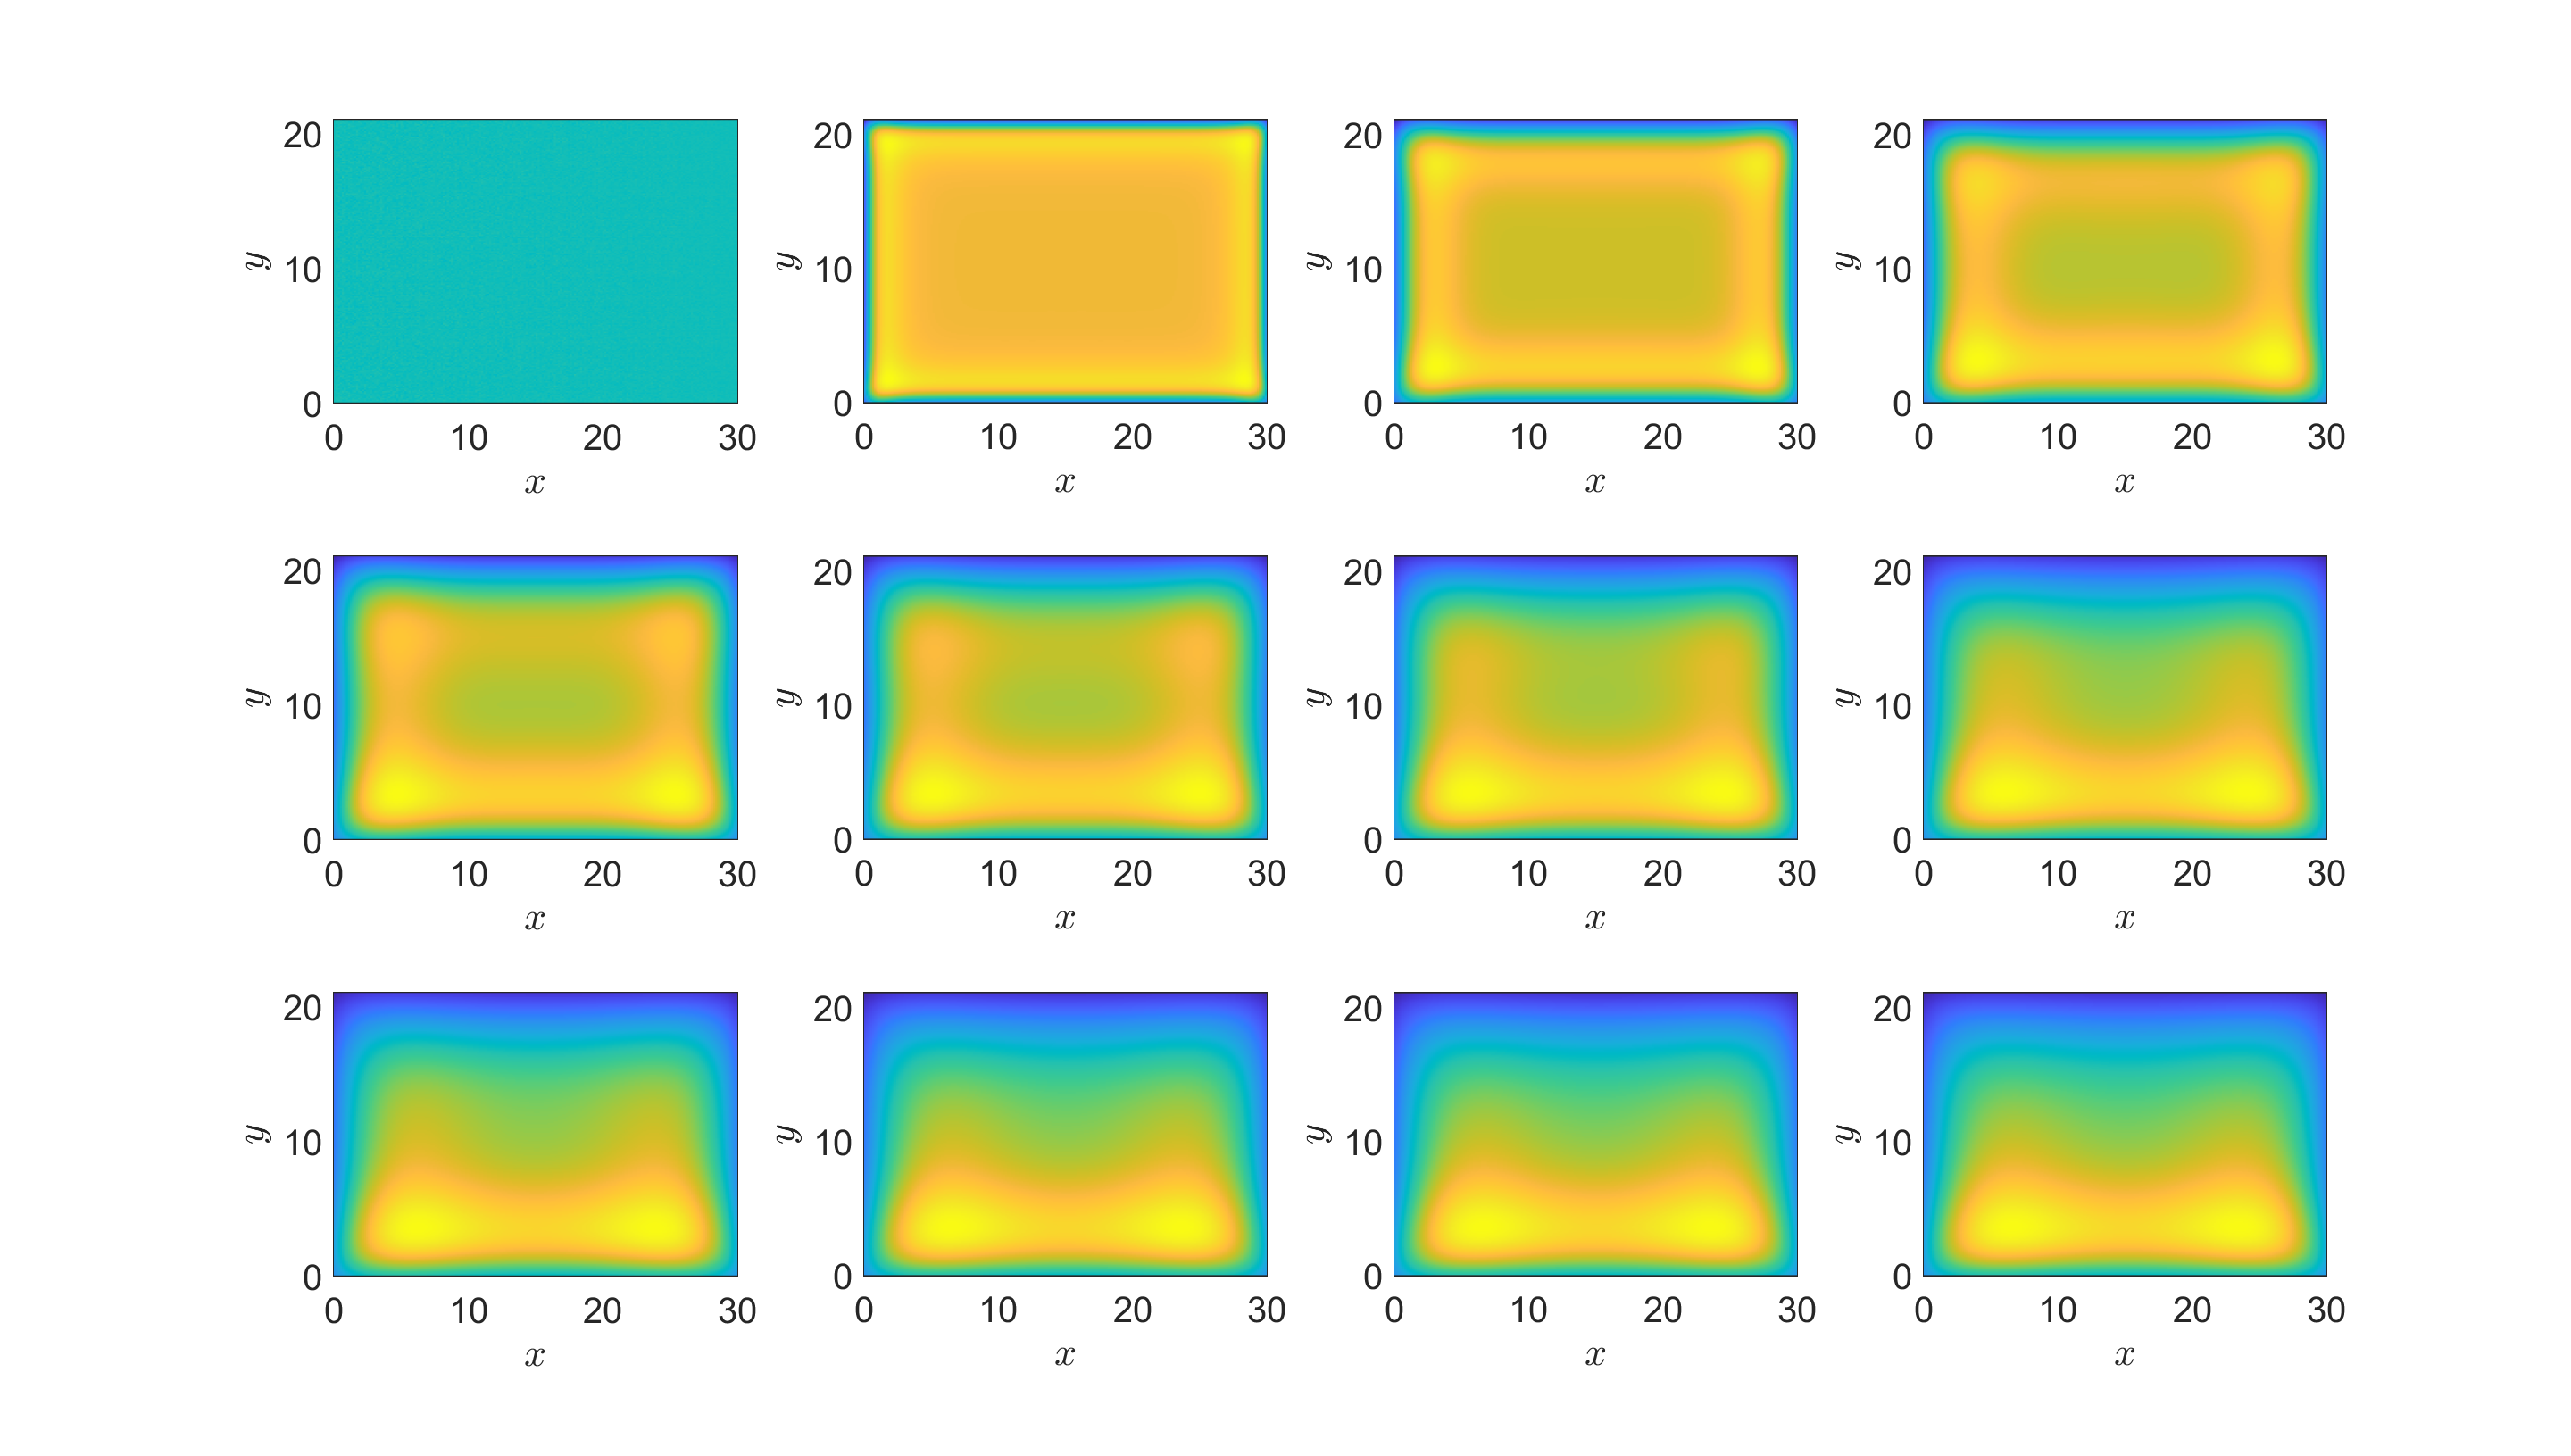
\includegraphics[scale=0.25]{SedOpt1.png}
	\caption{Optimal $\rho$} 
	\label{F3a}
	\end{figure}
	\begin{figure}[h]
	\centering
	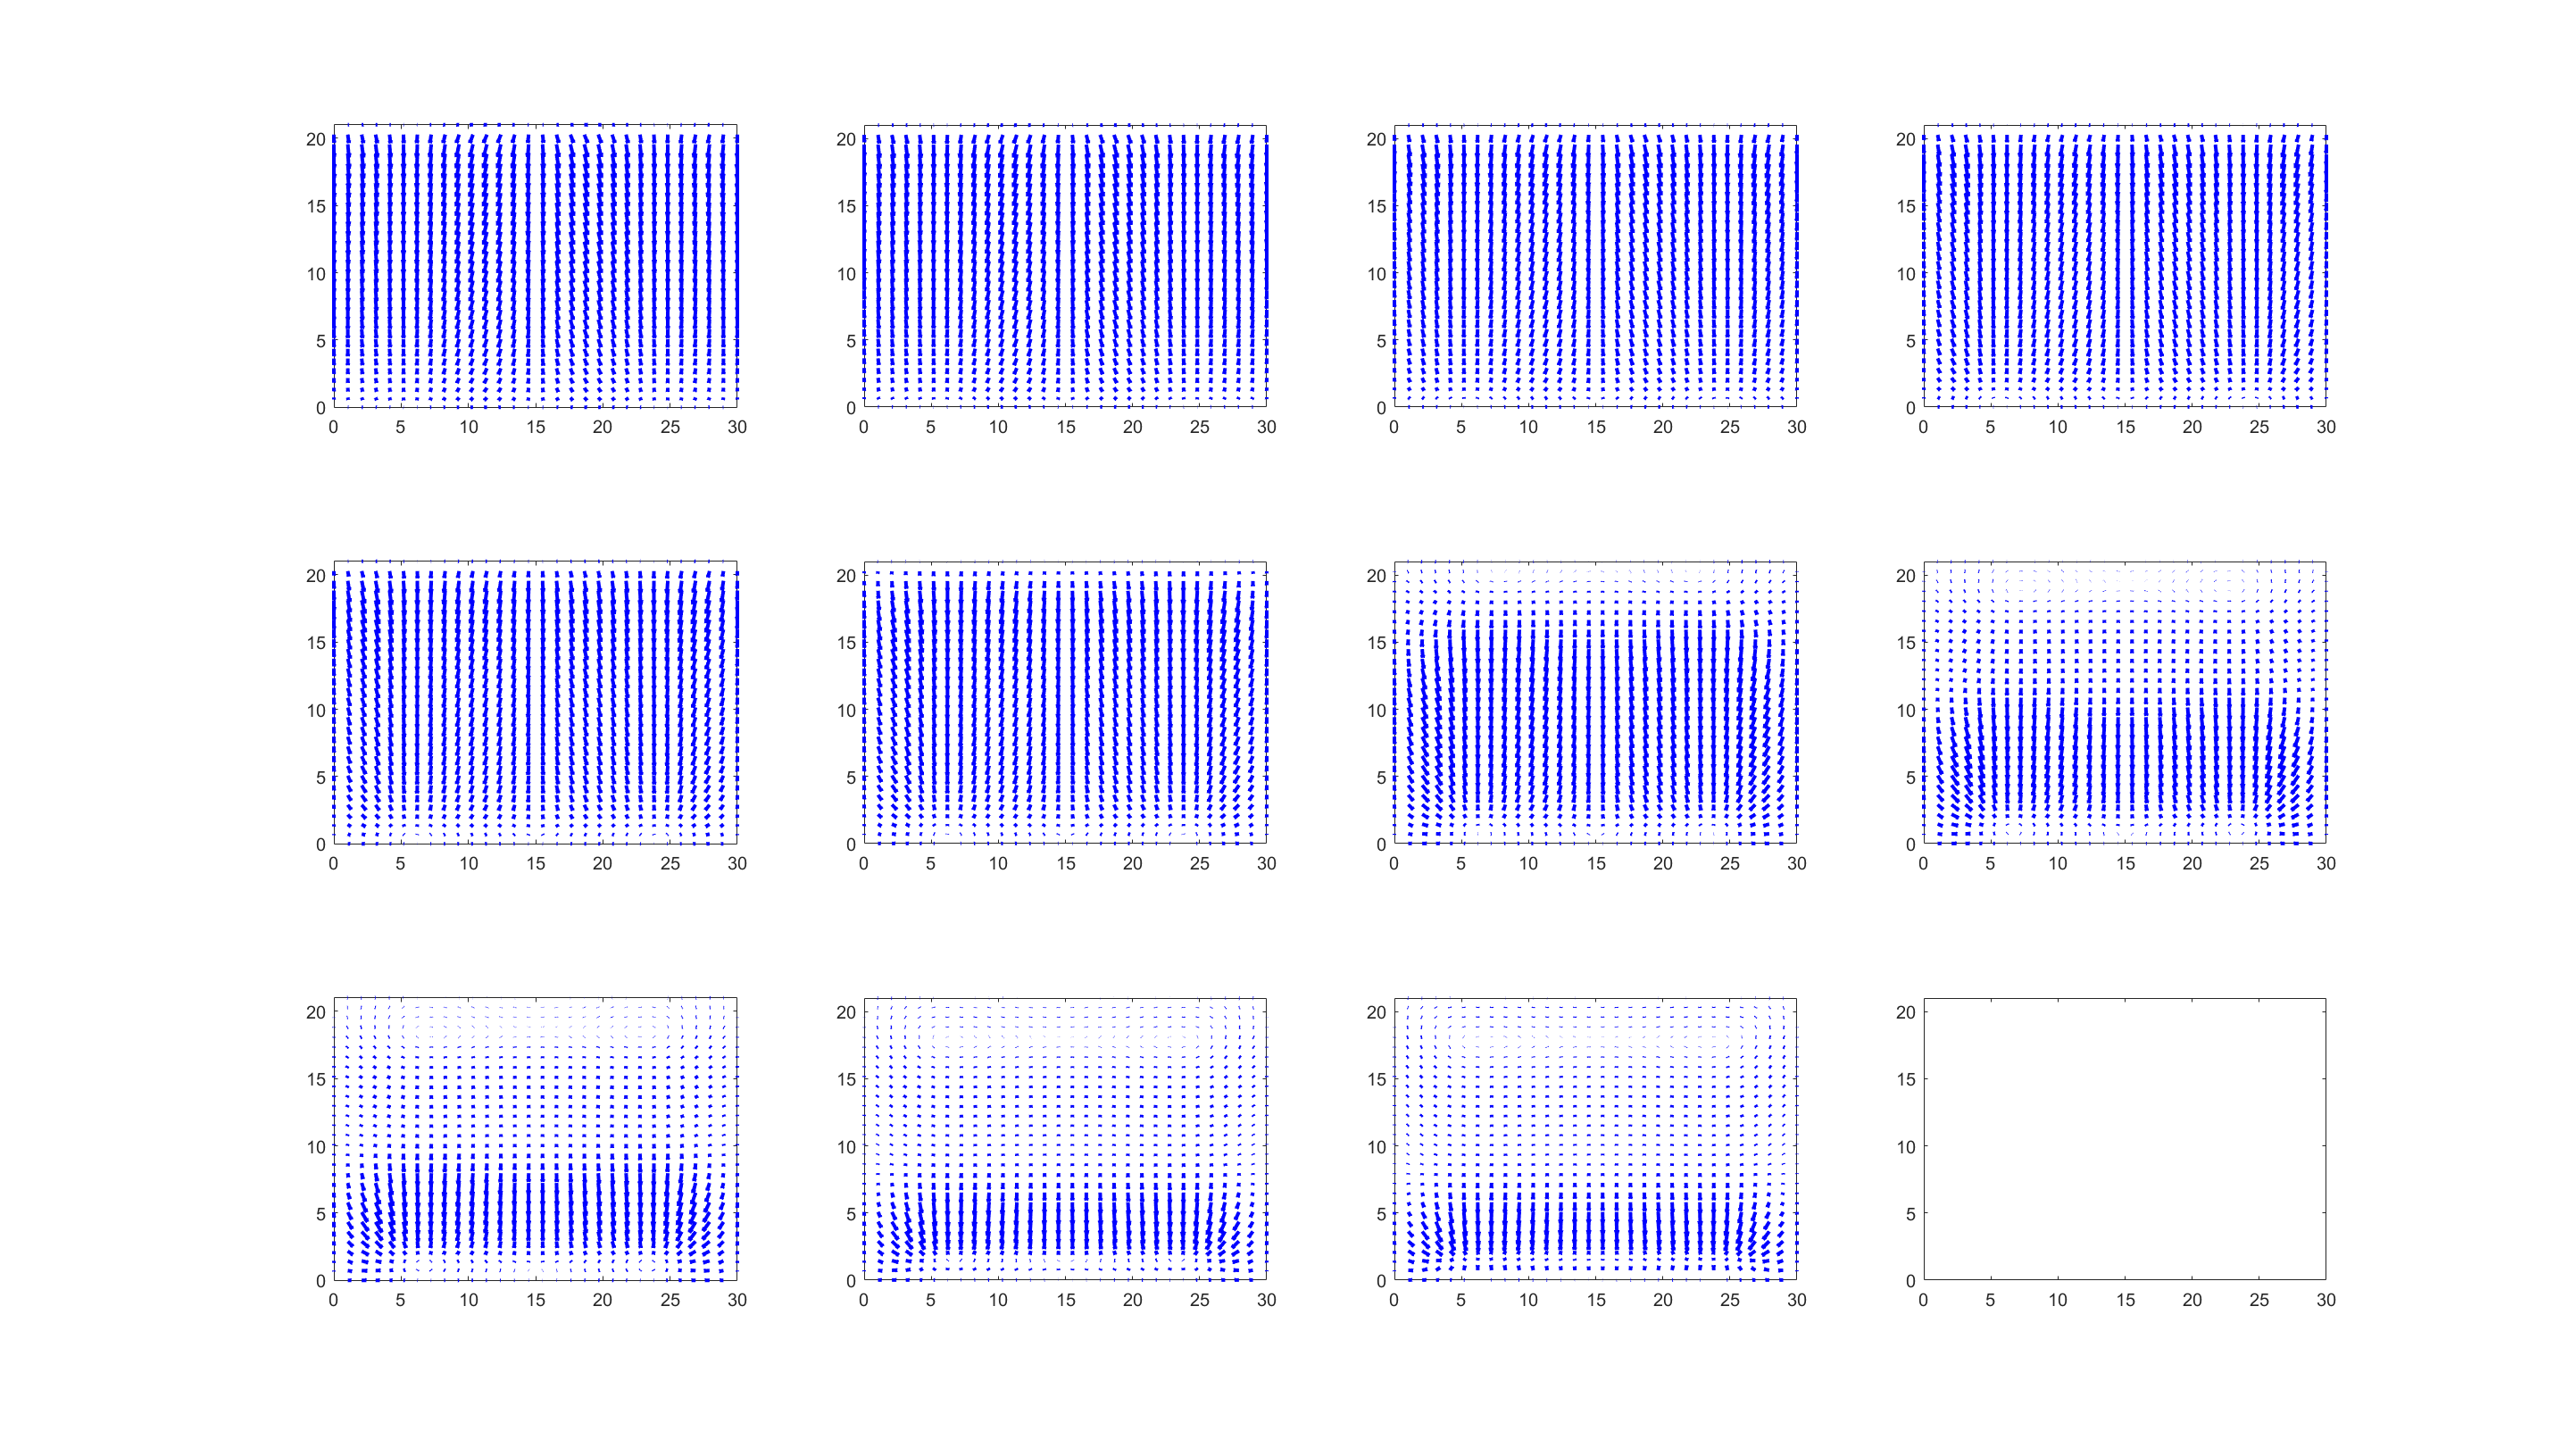
\includegraphics[scale=0.25]{SedOpt2.png}
	\caption{Optimal Control} 
	\label{F3b}
	\end{figure}

\end{document}